
%----------------------------------------------------------------------------------------
%   PACKAGES AND OTHER DOCUMENT CONFIGURATIONS
%----------------------------------------------------------------------------------------

% latexmk -pvc -pdf
\documentclass[12pt, a4paper]{report}
\usepackage[margin=2.5cm]{geometry}
\usepackage{titling}
\usepackage{titlesec}
\usepackage{amsmath,amsthm,amsfonts,amssymb}
\usepackage{mathtools}
\usepackage{braket}
\usepackage{dsfont}
\usepackage[font=scriptsize,labelfont=bf]{caption}
\usepackage[english]{babel}
\usepackage{graphicx}
\newenvironment{Figure}
    {\par\medskip\noindent\minipage{\linewidth}}
    {\endminipage\par\medskip}
\usepackage{tabularx}

% Colours:
\usepackage[table]{xcolor}
\definecolor{purple}{RGB}{117,77,226}

\usepackage[bookmarksopen,
  pagebackref,
  pdfpagelayout=TwoPageRight,
  colorlinks=true,
  urlcolor=purple,
  citecolor=purple,
  filecolor=purple,
  linkcolor=purple,
  urlcolor=purple,
  citecolor=purple,
  filecolor=purple,
  linkcolor=purple,
  linktocpage=true
  ]
{hyperref}

\titleformat{\chapter}[display]
  {\normalfont\bfseries}{}{0pt}{\Huge}

\newcommand\II{\(\mathcal{I}\)}
\newcommand\PT{\(\mathcal{PT}\)}
\newcommand\PP{\(\mathcal{P}\)}
\newcommand\TT{\(\mathcal{T}\)}
\newcommand\CPT{\(\mathcal{CPT}\)}
\newcommand\CC{\(\mathcal{C}\)}


\begin{document}
\begin{titlingpage}
  \begin{center}
  \vspace{2cm}
  {\Huge \( \mathcal{PT} \)-symmetric quantum mechanics}\\
  \vspace{0.5cm}
  \textsc{Honours Literature review}\\
  \vspace{1cm}
  {\Large Ana Fabela Hinojosa\\Student ID: 27876594}\\
  \vspace{0.5cm}
  {\Large Supervisors:\\ Dr. Jesper Levinsen \\ Prof. Meera Parish}\\
  \textsc{School of Physics \& Astronomy}\\
  \vspace{0.5cm}
  \includegraphics[scale=0.2]{logo.jpg} \\ % University logo
  {11th November 2022}\\
  \end{center}

  \begin{abstract}
  IN LESS THAN 100 WORDS

  % This work reflects on a possible extension to the canonical formalism of quantum mechanics. The main goal of this extension is to allow us to access a much larger class of interesting Hamiltonians which are non-Hermitian but nevertheless physically valid. This extension to quantum mechanics has the potential to be of great importance to the advancement of new and physically significant theories.


  %Quantum mechanical operators must satisfy a set of properties which deem them suitable as observable dynamical variables in nature. Observers use operators to measure some qualities of a system (such as for example a system's total energy) and come to a real valued finite answer.\\


  %However, all systems are always in contact with an environment, which often cannot be ignored or even defines the dominating influence on the system, e.g. gain and loss effects. In many cases a very elegant way of investigating open quantum systems with reasonable effort, in particular to avoid expensive time-dependent calculations, is made possible by non-Hermitian Hamiltonians.\cite{phdthesis}

% one should note that Hermiticity of the Hamiltonian is only a sufficient condition, which guarantees real eigenvalues and the conservation of probability densities. It needs to be emphasized that it is not a necessary condition and there could be non-Hermitian Hamiltonians with real discrete eigenvalue spectra, which then constitute potential candidates for physical applications, such as for instance atomic systems without decay \cite{Faria1}.

  \end{abstract}
\end{titlingpage}

\tableofcontents % Prints the main table of contents

%%%%%%%%%%%%%%%%%%%%%%%%%%%%%%%%%%%%%%%%%%%%%%%
\chapter{Introduction}\label{Introduction}
In ``The principles of quantum mechanics", Paul Dirac advises us that``it is important to remember that science is concerned only with \textit{observable} things and that we can observe an object only by letting it interact with some outside influence"\cite{POQM}. This means that in order to study valid physical systems, these systems must satisfy the fundamental postulates of quantum mechanical theory. Nearly all these postulates are based in physical properties. For example, one postulate establishes that time evolution of a quantum system must be \textit{unitary} (i.e. probability conserving). Another postulate requires that the energy spectrum of the system is bounded below so a lowest energy state can be measured. In quantum mechanics, the Hamiltonian operator $(\hat{H})$ encapsulates the total energy of a system. A system's energy spectrum is required to be bounded and real in order to be measurable. According to the fundamental postulates of the standard theory, if an operator $\hat{O}$ satisfies the mathematical property known as Hermiticity --these operators are also known as self-adjoint in mathematics-- then $\hat{O}$  has the property that its effect on the vectors of the Hilbert space in which $\hat{O}$ is defined is independent of the order in which $\hat{O}$ acts on said vectors\cite{Jones-Smith}
\begin{equation}\label{eq:1.1}
\hat{O}\ket{\psi} = \bra{\psi}\hat{O}^{\dagger}.
\end{equation}
Despite of the correctness of Hermiticity, some believe that perhaps we have ended up with an overly restrictive quantum theory. Therefore the aim of this review is to summarize the present developments of a quantum theory that uses an alternative postulate to Hermiticity. This alternative postulate is referred to as space–time reflection symmetry (\PT\:symmetry)\cite{MustaHbeHermitian}. 


%%%%%%%%%%%%%%%%%%%%%%%%%%%%%%%%%%%%%%%%%%%%%%%
\chapter{\texorpdfstring{$\mathcal{PT}$}\:-symmetry}\label{PT}
In the late nineties, Bender and Boettcher \cite{RealSpectrainNHH} presented a \PT-symmetric theory of quantum mechanics. Their aim was to explain a conjecture on the reality and positiveness of the spectrum of a non-Hermitian Hamiltonian proposed by Bessis, this Hamiltonian spectrum was surprising since it was widely thought that non-Hermitian Hamiltonians would not have physically valid energy spectra. In very general terms, \PT-symmetric theory can be viewed as an analytical continuation of the conventional theory from real into the complex phase space\cite{PTsymmetricQM}.

An important question that must be answered, is whether a \PT-symmetric Hamiltonian defines a valid physical theory of quantum mechanics. By a physical theory we mean that the following conditions must be satisfied; The energy spectra of a system described by $\hat{H}$ must be real and bounded below. Another condition is related to the probabilistic interpretation of the norm of a state, a norm must be always positive to be a valid probability. Finally, time evolution under the theory must be unitary. This means that as a state vector evolves in time the state's probability does not leak away\cite{MustaHbeHermitian}\cite{MakingSense}.

%%%%%%%%%%%%%%%%%%%%%%%%%%%%%%%%%%%%%%%%%%%%%%%
\section{The \texorpdfstring{$\mathcal{PT}$}\: operator}
The \PT\:operator is the anti-linear operator composed of the linear parity operator (\PP), which performs spatial reflection, and the anti-linear time-reversal operator (\TT). These operators act on position and momentum operators in the following form
\begin{equation}\label{eq:2.1}
\begin{split}
\mathcal{P}:& \quad\hat{x} \rightarrow -\hat{x},\quad \hat{p} \rightarrow -\hat{p},\\
\mathcal{T}:& \quad\hat{x} \rightarrow \hat{x},\quad\quad \hat{p} \rightarrow -\hat{p},\quad \mathrm{i} \rightarrow -\mathrm{i}
\end{split}.
\end{equation}
Some Hamiltonians may not be symmetric under \PP\:or \TT\:separately, but Hamiltonians that remain invariant under the influence of the \PT\:operator are labelled as \PT-symmetric. 
A Hamiltonian $\hat{H}$ will possess unbroken \PT\:symmetry if the following conditions are satisfied
\begin{equation}\label{eq:2.2}
[\tilde{H}, \mathcal{PT}] = 0\quad\mathrm{and}\quad\mathcal{PT}\ket{\psi_n} = \ket{\psi_n},
\end{equation}
where $\ket{\psi_n}$ are the eigenstates of $\tilde{H}$. The second condition in \ref{eq:2.2} means that the eigenstates $\ket{\psi_n}$ are simultaneously eigenstates of the \PT\: operator. Unfortunately, the anti-linearity of the \PT\:operator is responsible for the possibility that only the first identity in \ref{eq:2.2} could hold, but not the second\cite{Faria1}.
If both conditions in \ref{eq:2.2} hold then the \PT-symmetry of $\tilde{H}$ is unbroken. This means that the eigenspectrum of $\tilde{H}$ is fully real and bounded below --This is also known as exact \PT-symmetry--.
\begin{Figure}
\centering
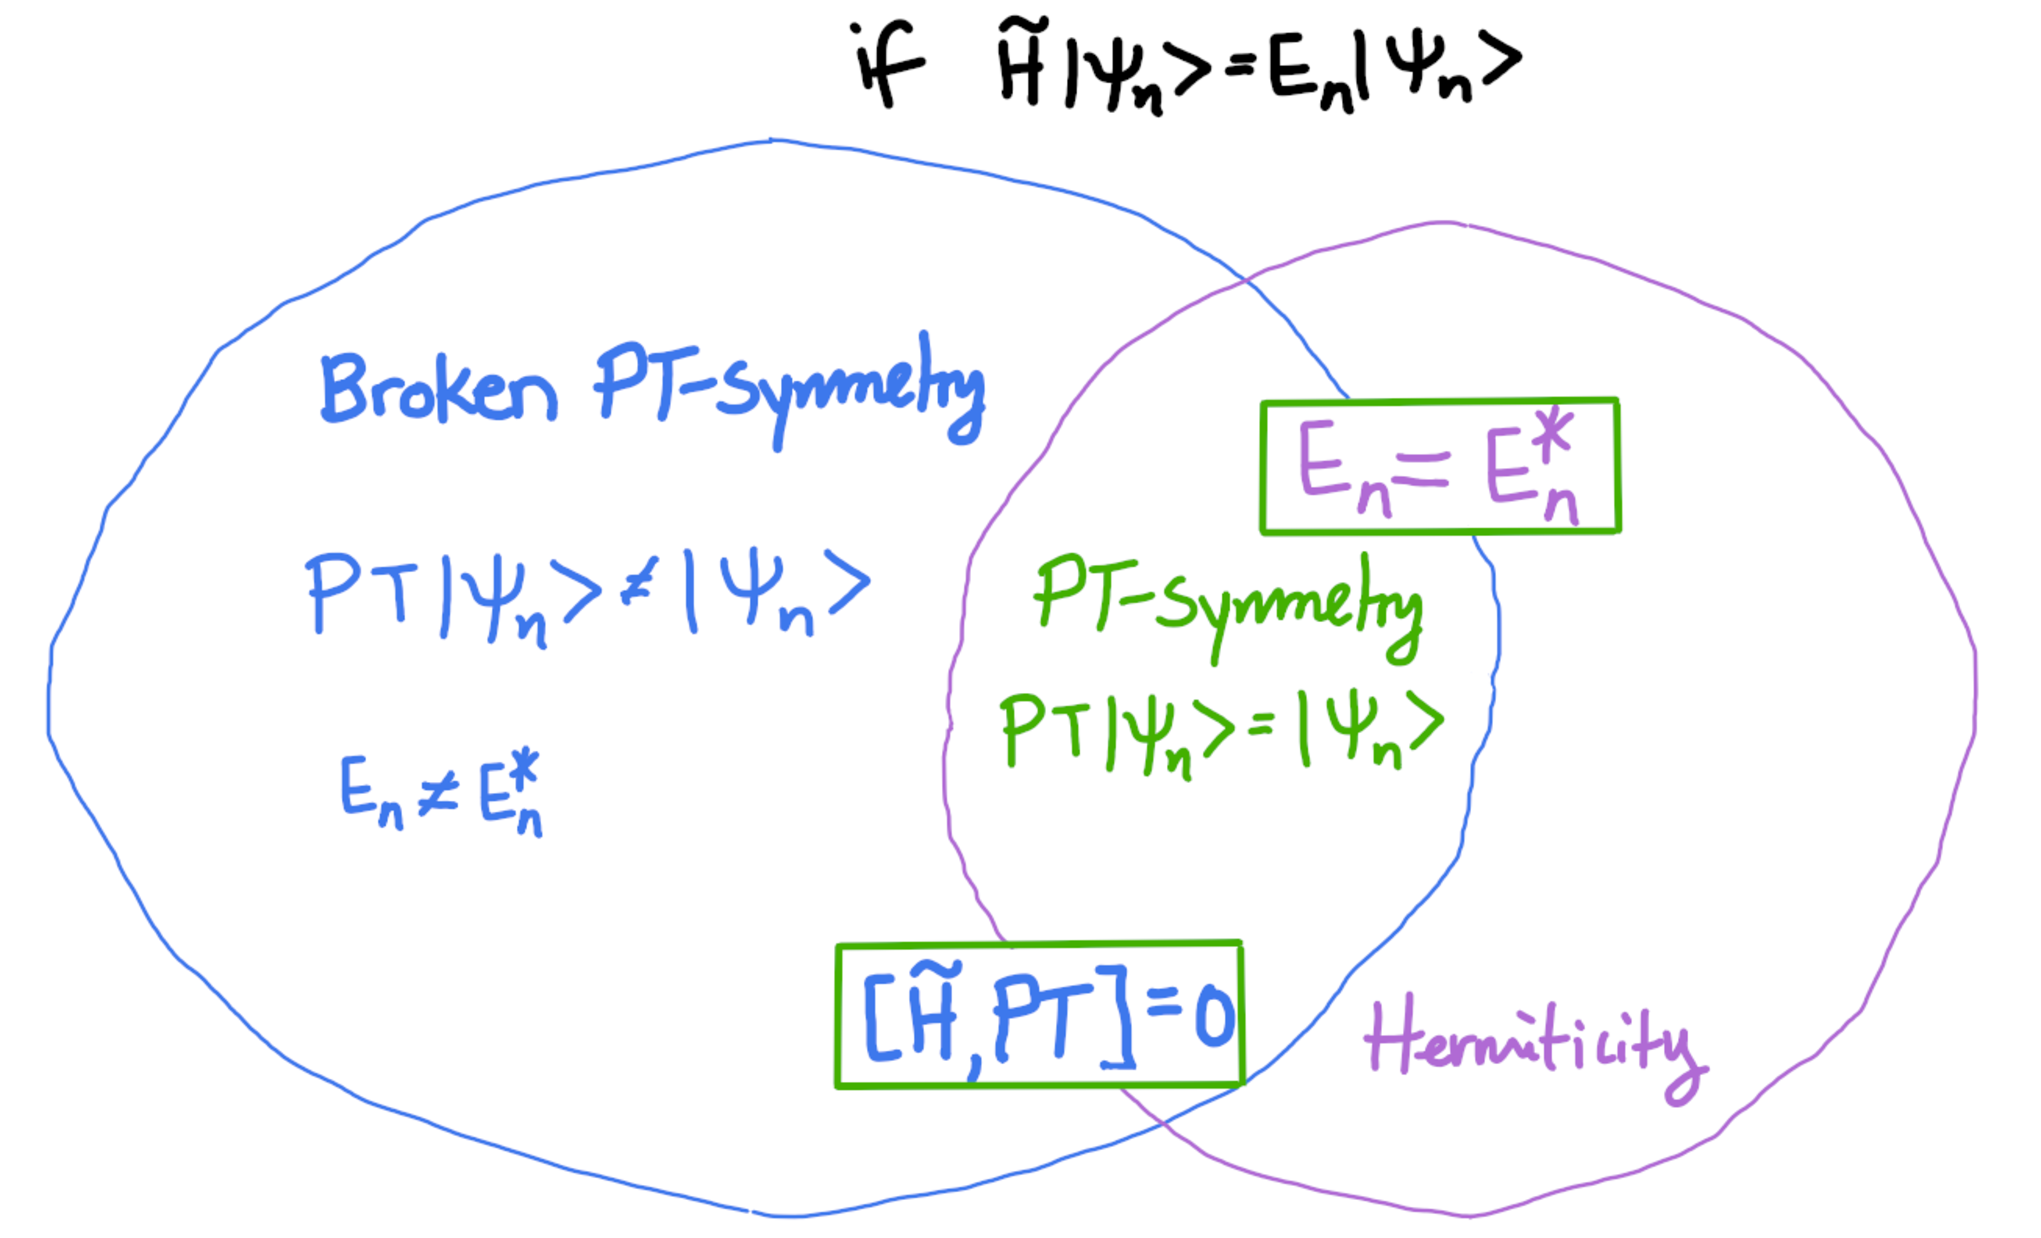
\includegraphics[width=0.7\linewidth]{eigenvalues_and_PTsymmetry.pdf}
\captionof{figure}{Illustration of the conditions in equations \ref{eq:2.2}. \PT-symmetry and the reality of eigenvalues. This figure is strongly inspired by figure 2 in reference \cite{Faria1}}
\label{fig:eigenvalues}
\end{Figure}
The effectiveness of \PT\:symmetry as a tool to investigate the spectra of some non-Hermitian Hamiltonians has been shown in various works, such as Dorey et al\cite{Dorey_2001}, Bender and Boettcher\cite{Bender1998}, Brody\cite{Brody_2016}, Bender and Mannheim \cite{Bender_2010}, Bender et al\cite{PTsymmetricQM}, Mostafazadeh\cite{Mostafazadeh}\cite{Mostafazadeh2} amongst others. 

To ensure that a the eigenstates $\{\ket{\psi_n}\}$ of a \PT-symmetric Hamiltonian $\tilde{H}$ are orthogonal, it is necessary to specify an inner product. A possible choice for the inner product associated with $\tilde{H}$ might be\cite{PTsymmetricQM}
\begin{equation}\label{eq:2.3}
\braket{\psi_n|\psi_m} \equiv \int_{c} dx [\psi_{n}(x)]^{\mathcal{PT}}\psi_m(x) = \int_{c} dx [\psi_{n}(-x)]^{*}\psi_m(x)
\end{equation}
where $c$ is a complex contour that starts and ends within specific boundary conditions (see section \ref{App4}). Unfortunately this obvious choice for the \PT\:inner product is not correct because it does not guarantee a positive definite norm.

%%%%%%%%%%%%%%%%%%%%%%%%%%%%%%%%%%%%%%%%%%%%%%%
\section{The \texorpdfstring{$\mathcal{CPT}$}\:\:inner product}\label{CPT}
To be able to describe precisely the nature of \PT-symmetric quantum mechanics, we must delve briefly into the inner-product under which our theory satisfies the postulates of conventional quantum mechanics. It is important to note that \PT-symmetric quantum mechanics is a kind of `bootstrap' theory\cite{MakingSense}, since infinitely many inner-products exist for a given vector space, we can construct an inner product whose associated norm is positive definite by design. This inner-product is in general dependent on the characteristics of the Hamiltonian in question and it guarantees that the underlying dynamics of any \PT-symmetric Hamiltonian satisfies unitarity\cite{MustaHbeHermitian}.
Firstly, it is necessary to solve for the eigenstates of the Hamiltonian before knowing the Hilbert space and consequentially the associated inner product.
To guarantee a positive norm for our theory, we will construct a new linear operator \CC\:that commutes with both $\hat{H}$ and \PT. We use the symbol \CC\: to represent this symmetry because it's properties are similar to those of the charge conjugation operator in particle physics\cite{MakingSense}.

%%%%%%%%%%%%%%%%%%%%%%%%%%%%%%%%%%%%%%%%%%%%%%%
\subsection{The $\mathcal{C}$ operator}\label{CC}
When the \PT-symmetry of $\hat{H}$ is unbroken, then $\hat{H}$ and \PT\:commute. This statement is equivalent to saying that the eigenfunctions $\phi_n(x)$ of $\hat{H}$ are simultaneously eigenstates of the \PT\:operator\cite{Bender_2004}
\begin{equation}\label{eq:2.4}
\mathcal{PT}\phi_n(x) = \lambda_n \phi_n(x),
\end{equation}
Where $\lambda_n$ is a pure phase. Without loss of generality, for each $n$\:the phase can be absorbed into $\phi_n(x)$ and this makes the eigenvalue of the \PT operator unity\cite{Bender_2004}: 
\begin{equation}\label{eq:2.5}
\mathcal{PT}\phi_n(x) = \phi_{n}^{*}(-x) = \phi_n(x).
\end{equation}

There is strong numerical evidence of the completeness of the eigenfunctions $\phi_n(x)$\cite{ComplexExtension}\cite{Bender_2004}\cite{Brody_2013}. In the coordinate basis, the completeness statement reads:
\begin{equation}\label{eq:2.6}
\sum_{n}(-1)^{n}\phi_n(x)\phi_n(y) = \delta(x-y),\quad x, y \in \mathbb{R}
\end{equation}
the unconventional $(-1)^n$ factor in \ref{eq:2.6} can be explained if we define the \PT\:inner product as
\begin{align}\label{eq:2.7}
\left ( f, g \right )  & = \int dx \left [ \mathcal{PT} f(x) \right ] g(x)\nonumber\\
                       & = \int dx f^{*}(-x) g(x).
\end{align}
where the integral above follows a path in the complex plane. Under this definition the eigenstate norms alternate in sign depending on the value $n$. This means that the metric associated with the \PT\: inner product is indefinite\cite{Bender_2004}\cite{Critique}.
In quantum theory, the norm of states is interpreted as a probability and this means that the indefinite metric described above presents a serious problem for the validity of \PT-symmetric quantum theory. The solution to this problem lies in finding an interpretation for the negative valued norms\cite{PTsymmetricQM}.

Most model \PT-symmetric Hamiltonians $\tilde{H}$ in the literature admit tuneable parameters such that there will be regions in the parameter space where the eigenstates of $\tilde{H}$ are not \PT-symmetric\cite{Brody_2013}. This means that a system described by $\tilde{H}$ admits two phases, one for broken and another for unbroken \PT-symmetry. In the unbroken phase eigenstates of $\tilde{H}$ become degenerate and this implies that they lose completeness\cite{Brody_2013}. 

The literature claims that for any theory with unbroken \PT-symmetry there exists a symmetry of the Hamiltonian that describes the negative and positive norm states. To describe this symmetry of $\hat{H}$ it is necessary to construct a linear operator denoted by \CC\cite{MustaHbeHermitian}\cite{ComplexExtension}\cite{Bender_2004}. When represented in position space \CC\: is a sum over the energy eigenstates of $\hat{H}$:
\begin{equation}\label{eq:2.8}
\mathcal{C} = \sum_n \phi_n(x)\phi_n(y)
\end{equation}
From this definition, and from the relation $(\phi_m(y), \phi_n(y)) = \int dy\:\phi_m(y)\phi_n(y)$ we can verify that the eigenvalues of \CC\: are $\pm 1$
\begin{align}\label{eq:2.9}
\mathcal{C} \phi_n(x) & = \int dy\:\mathcal{C}\:\phi_n(y)\nonumber \\
& = \sum_{m}\phi_m(x)\int dy\:\phi_m(y) \phi_n(y)\nonumber \\
& = (-1)^n \phi_n(x)
\end{align}
The \PT\:norm signatures can therefore be interpreted as the ``charge'' of the states, while \CC\: is the operator used to measure this charge\cite{Bender_2004}.

The \CC\: operator commutes with the \PT\: operator, but it does not commute with the parity operator \PP. Notice that \CC\:and \PP\: operators are square roots of $\delta(x-y)$ the unity operator\cite{ComplexExtension}
\begin{equation}\label{eq:2.10}
\mathcal{P}^2 = \mathcal{C}^2 = \mathds{1}, 
\end{equation}
where $\mathcal{P} \neq \mathcal{C}$, since \PP\: is real and \CC\: is complex valued\cite{MustaHbeHermitian}\cite{Bender_2004}.

Using the newly constructed \CC\: operator, we can redesign the \PT\: inner product to suit the conventional probabilistic interpretation of the vector norms in quantum mechanics
\begin{equation}\label{eq:2.11}
\left( f, g \right ) = \int dx \left [ \mathcal{CPT} f(x) \right ] g(x).
\end{equation}

\section{$2\times2$ \PT-symmetric Hamiltonian}
An example of the results of unbroken \PT-symmetric theory that is often found in the literature describes a simple finite non-Hermitian but \PT-symmetric Hamiltonian
\begin{equation}\label{eq:2.12}
\tilde{H} = \begin{pmatrix}
re^{i\theta} & s  \\
s & re^{-i\theta} \\
\end{pmatrix}
\end{equation}
where the parameters $r, s$ and $\theta$ are real. In this setup the \TT\: operator performs complex conjugation and the parity operator is written as
\begin{equation}\label{eq:2.13}
\mathcal{P} = \begin{pmatrix}
0 & 1  \\
1 & 0 \\
\end{pmatrix}.
\end{equation}
The Hamiltonian in \ref{eq:2.12} allows two parametric regions. When $s^2 < r^2\sin^2\theta$ the eigenvalues of $\tilde{H}$ form a complex conjugate pair. This is the broken \PT-symmetry region. Otherwise, when $s^2 \geq r^2\sin^2\theta$, then the eigenvalues are real. This is the region of unbroken \PT-symmetry region. In the unbroken symmetry region the \PT\: normalised eigenstates of both $\tilde{H}$ and \PT\: are
\begin{equation}\label{eq:2.14}
\ket{E_{+}} = \frac{1}{\sqrt{2\cos\alpha}}\begin{pmatrix}
e^{i\alpha/2} \\
e^{-i\alpha/2} \\
\end{pmatrix}\quad\mathrm{and}\quad\ket{E_{-}} = \frac{i}{\sqrt{2\cos\alpha}}\begin{pmatrix}
e^{-i\alpha/2} \\
-e^{i\alpha/2} \\
\end{pmatrix},
\end{equation}
we use the relation $\sin\alpha = \frac{r}{s}\sin\theta$.
The corresponding \CC operator for this Hamiltonian is 
\begin{equation}\label{eq:2.15}
\mathcal{C} = \frac{1}{\cos\alpha}\begin{pmatrix}
i\sin\alpha & 1 \\
1 & -i\sin\alpha\\
\end{pmatrix},
\end{equation}
This \CC\: operator commutes with $\tilde{H}$ and satisfies $\mathcal{C}^2= \mathds{1}$. The eigenvalues of \CC\:are precisely the signs of the \PT\:norms of the corresponding eigenstates\cite{Bender_2004}. Using this \CC\: operator we can guarantee that the \CC\PT inner product in the two-dimensional Hilbert space spanned by $\ket{E_{\pm}}$ is positive definite.

%%%%%%%%%%%%%%%%%%%%%%%%%%%%%%%%%%%%%%%%%%%%%%%%%%%%%%%%%%%%%%%%%%%%%%%%%%%%%%%
\chapter{Time evolution}\label{Tev}
In Hermitian quantum mechanics, time-evolution of states is done by using the unitary operator $\hat{U} = e^{-i\hat{H}t/\hbar}$. Because the $\hat{U}$ operator is unitary this means that as the state $\vec{\psi}$ evolves in time, its norm remains constant. This is useful in quantum mechanics because the norm of a state is interpreted as a probability, and therefore unitarity guarantees that a state's probability does not grow or decay with time. As explained in section \ref{CPT}, when the \PT-symmetry of $\hat{H}$ is unbroken it is possible to have positive definite \CPT norm states for the non-Hermitian Hamiltonian. This means that time evolution under the unbroken \PT-symmetric framework is also unitary\cite{Jones-Smith}\cite{ComplexExtension}\cite{Mostafazadeh2}. 
The unitary time evolution of a state $\vec{\psi}$ from time $t = 0$ to a time $t$ is written as
\begin{equation}\label{eq:3.1}
\vec{\psi}(t) = \hat{U} \vec{\psi}(0),
\end{equation}
We can be put aside Hamiltonians with unbroken \PT-symmetry for the time being since states under these undergo trivial dynamics.

\section{Time evolution under broken \PT-symmetry}
In contrast with unbroken symmetry, Hamiltonians with broken \PT-symmetry do not satisfy the spectral theorem and this gives rise to very unconventional quantum mechanical behaviour. Hamiltonians with broken \PT-symmetry exhibit purely non-Hermitian spectral degeneracies known as exceptional points (EP)\cite{Bossart}. EPs are points in an (at least) two-dimensional parameter space, in which two or more eigenstates become identical\cite{Moiseyev}\cite{Cartarius}. 
The interest in these degeneracies has increased greately since they give rise to dramatic effects in a great variety of physical problems: in mechanics, electromagnetism, atomic and molecular physics, quantum phase transitions, quantum chaos and more\cite{Heiss_2012}.

An illustrative example of EPs can be seen when we consider the well known family of \PT-symmetric Hamiltonians
\begin{equation}\label{eq:3.2}
\hat{H} = \hat{p}^2 + \hat{x}^{2}(i x)^{\epsilon} \quad\quad (\epsilon\:\mathrm{real}). 
\end{equation}
These Hamiltonians have unbroken \PT\:symmetry when $\epsilon \geq 0$ and broken \PT-symmetry when $\epsilon < 0$. The energy spectrum of \ref{eq:3.1} has been proved to be real and bounded below in the region of unbroken \PT\:symmetry \cite{Dorey_2004}. In figure \ref{fig:parametricfam} both these regions and the phase transition the spectrum are visible.
\begin{Figure}
\centering
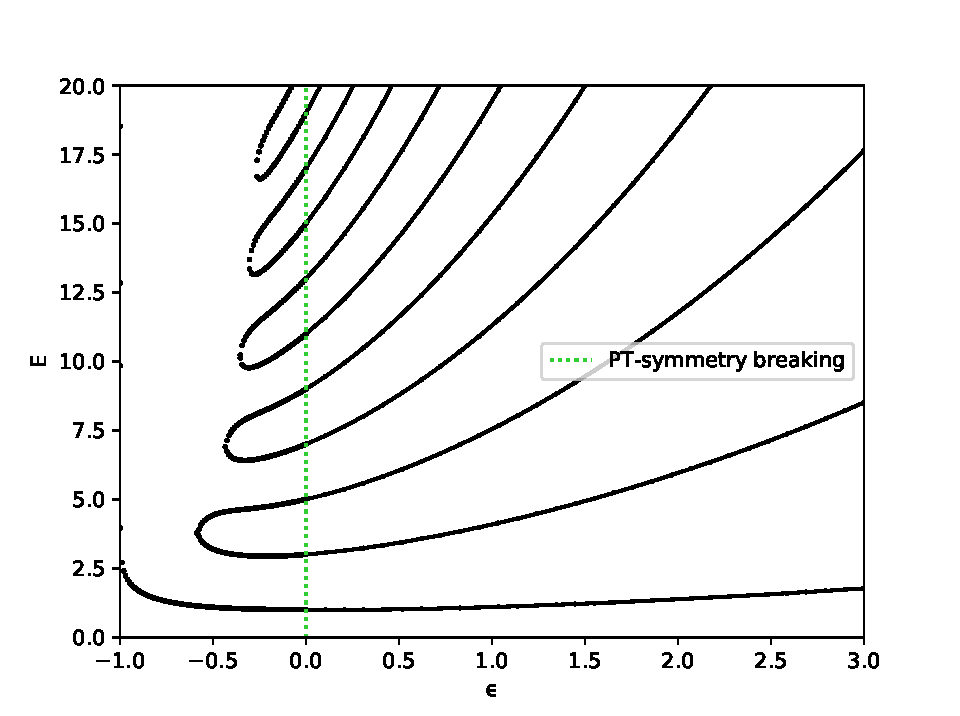
\includegraphics[width=0.7\linewidth]{parametric_fam.pdf}
\captionof{figure}{This figure is my version of Figure 1. in reference \cite{MakingSense}, it exemplifies the behaviour of the eigenvalue spectra of the Hamiltonians in \ref{eq:3.1} as a function of the real parameter $\epsilon$. All the eigenvalues visible in this figure are real valued. The vertical dotted green line corresponds to the value $\epsilon = 0$, this is the point where \PT-symmetry breaks and it corresponds to the Hamiltonian for the classic one dimensional harmonic oscillator. When $\epsilon \geq 0$ the spectra are real, positive and discrete. Energy levels increase with increasing $\epsilon$. In the region corresponding to $-1 \leq \epsilon \leq 0$ there is a finite number of real positive eigenvalues and an infinite number of complex-conjugate pairs of eigenvalues (not depicted). The number of real eigenvalues decreases as $\epsilon$ decreases from $0$ to $-1$, for $\epsilon$ that are more negative than the value $\epsilon = -0.57793$ the only remaining real eigenvalue corresponds to the ground-state energy. At the value $\epsilon = -1$ the spectrum is null  as all eigenvalues diverge towards positive infinity.}
\label{fig:parametricfam}
\end{Figure}
In chapter \ref{MINE} we will investigate the unbroken symmetry region of figure \ref{fig:parametricfam}, specifically the case for $\epsilon = 2$. However since in this section we are concerned with EPs, we must zoom into the parametric region $\epsilon < 0$, that is the broken \PT-symmetry region.
\begin{Figure}
\centering
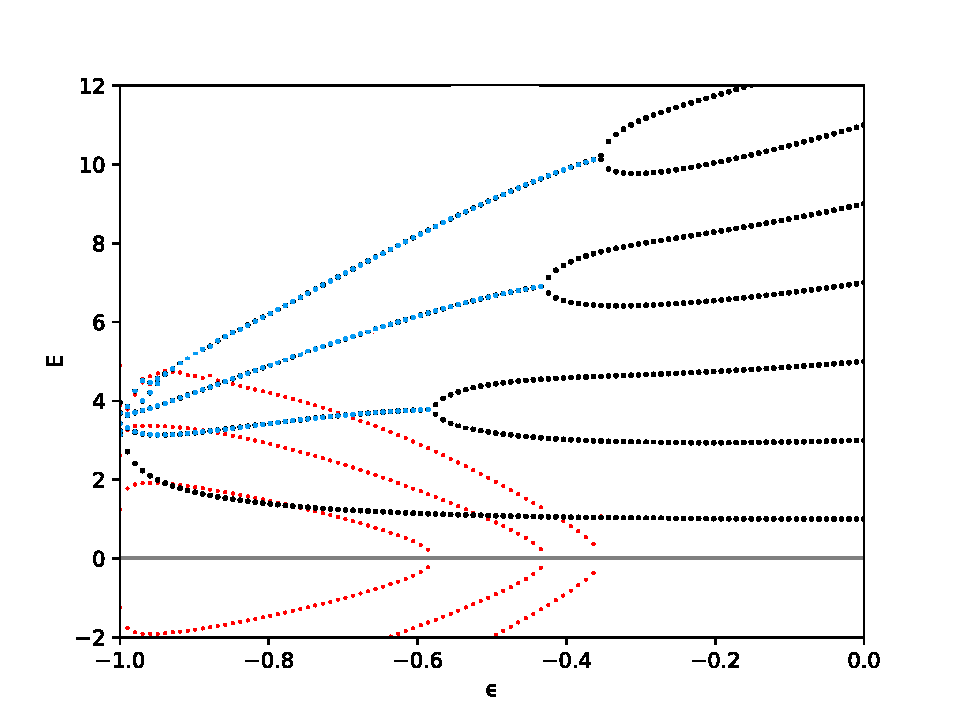
\includegraphics[width=0.7\linewidth]{broken_region.pdf}
\captionof{figure}{This figure is my version of Figure 3. in reference \cite{BrokenRegion}, it exemplifies the behaviour of the eigenvalue spectra of the Hamiltonians in \ref{eq:3.1} as a function of the real parameter $\epsilon$ in the case where $\epsilon < 0$. This figure displays a discretised  parameter space for $\epsilon$ as 100 values in the horizontal axis, and the eigen-energy range $-2 \leq E \leq 12$ as the vertical axis. This figure depicts fully real eigenvalues as black dots. Visible here are three epsilon values at which the real eigenvalues become degenerate (coalesce) and then form complex-conjugate pairs. The real parts of these pairs of eigenvalues are represented as blue dots. These energies initially decrease as $\epsilon$ decreases but blow up suddenly as $\epsilon$ approaches $-1$ (The blow up of the real-parts was not captured by my numerics). The imaginary parts of the eigenvalue pairs are represented as red dots. These remain finite and appear to decay to zero at $\epsilon = -1$.}
\label{fig:broken_region}
\end{Figure}
In figure \ref{fig:broken_region} above, we can see three distinct EPs of order one.


\subsection{Time evolution at the exceptional point}\label{EPs}



% may incorporate complex potentials that result in the decay or growth of the probability densities of wavefunctions. This feature can be useful for implementing reflection-free absorbers at the boundaries of wave simulations\cite{Moiseyev}\cite{Cartarius}. However, since these Hamiltonians


% the role of EP encircling and the importance of the modulation
% details (speed, strength, center) is still not well understood.
% A general theory and classification of static and Floquet non-
% Hermitian time-evolution is still missing and crucial to under-
% stand the interplay between the static non-Hermitian proper-
% ties of the unmodulated system and periodic dynamic modu-
% lation\cite{Cartarius}.



\section{Faster than Hermitian time evolution?}\label{faster}
It has been suggested in \cite{Bender_2007} that it is possible to obtain arbitrarily fast quantum evolutions using non-Hermitian \PT-symmetric Hamiltonian operators. This is because for such Hamiltonians the path from can be made short. 
The mechanism described in \cite{Bender_2007} is similar to that in general relativity in which the distance between two space-time points can be made small if they are connected by a wormhole. If true, The results in \cite{Bender_2007} will have drastic consequences in quantum computation, because it removes the bound on the time-optimal unitary NOT operations\cite{OptimalControl} that is obtained in quantum mechanics\cite{Brachistochrone_Mostafazadeh}. However, Bender et al warn us about the possibility of the existence of quantum protection mechanisms that place a lower bound on the time required to switch Hilbert spaces. which would limit the applicability of a Hilbert-space ``wormhole" to improve quantum algorithms\cite{Bender_2007}. 

G\"{u}nther and Samsonov have interpreted the \PT-symmetric setup for \cite{Bender_2007} as a quantum system
consisting of a non-Hermitian \PT-symmetric component and a Hermitian component simultaneously. In \cite{Gunther_2008} G\"{u}nther and Samsonov formulate a general recipe for the construction of partially \PT-symmetric quantum
systems which are not 1:1 equivalent to purely Hermitian systems. Using a strong structural analogy with the
reference frames for inertial observers in special relativity, they associate \PT-symmetric models in different
representations with corresponding measurement frames. They claim that the resultant operators which are Dirac Hermitian
are connected with non-Dirac-Hermitian operators in another frame. The probabilistic content of the models
is frame-independent. According to G\"{u}nther and Samsonov their geometric analysis of the equivalence mapping between mutually \PT-symmetric and Hermitian operators demonstrates the agreement of the vanishing passage-time solution proposed in \cite{Bender_2007} and the temporal lower bound for Hermitian evolution proposed by Anandan and Aharonov in \cite{AnandanAharonov}. 

Despite the potential importance of \PT-symmetric theory, the experimental observation in a genuine quantum system is still missing\cite{Cartarius}.
Therefore, the purpose of our research is determine whether a realistic \PT-symmetric quantum system and its dynamics can be potentially accessible in an experiment. 

%%%%%%%%%%%%%%%%%%%%%%%%%%%%%%%%%%%%%%%%%%%%%%%%%%%%%%%%%%%%%%%%%%%%%%%%%%%%%%%
% \chapter{Experiments}

% Much research has been carried out on properties of physical systems described by \PT-symmetry. Such Hamiltonians can be used to model the behavior of closed quantum systems, but they can also be replicated in open systems which exhibit balanced gain and loss, and this has been implemented in laboratory experiments for a wide range of systems\cite{geometric_aspects}.  



\chapter{Project statement}\label{MINE}
We are concerned with the dynamical processes of non-Hermitian systems. Specifically we are interested in understanding the behaviour of quantum mechanical superfluids in non-Hermitian traps. Our ultimate goal in this project is the experimental observation of the dynamics of a Bose-Einstein condensate in a one dimensional Hermitian potential as a quench transforms the potential into a \PT-symmetric trap in the shape of an inverted quartic in one dimension.

In section \ref{Eps} we investigated the well known parametric family of \PT-symmetric Hamiltonians in \ref{eq:3.1}. As explaine previously, these Hamiltonians have unbroken \PT\:symmetry when $\epsilon \geq 0$ and broken \PT-symmetry when $\epsilon < 0$. The particular Hamiltonian that we use in my project occurs when we let $\epsilon = 2$ in \ref{eq:3.1}, leaving us with 
\begin{equation}\label{eq:}
\hat{H} = \hat{p}^2 - \hat{x}^{4};
\end{equation}
this Hamiltonian is interesting because even though it posseses an upside-down potential, it nevertheless appears to have a fully real and bounded below energy spectrum\cite{UpsideDownPotentials} as can be seen in figure \ref{fig:parametricfam}. Our present aim is to simulate the dynamics of a trapped state after we implement a quench that would instantaneously change the trapping potential from a harmonic oscillator trap to the inverted quartic potential in \ref{eq:}.


\section{Investigating \PT-symmetric time evolution}
Here I include some of the progress I made in my work on the dynamics under the \PT-symmetric Framework. 
% For $\tilde{H}$ whose eigenvectors span the Hilbert space $\mathcal{H}$\cite{Bender_2007}. Without loss of generality, since we are dealing with a two-level system, it is useful to use the Bloch sphere to visualise the geometry of this system. Let the eigenvectors of $\tilde{H}$ be
% \begin{align}\label{eq:1.13}
% \ket{\psi_{i}} = \begin{pmatrix}
% 1\\
% 0\\
% \end{pmatrix}, \quad\ket{\psi_f} = \begin{pmatrix}
% 0\\
% 1\\
% \end{pmatrix}.
% \end{align}
% There are many possible paths for the time evolution from $\ket{\psi_{i}}$ to $\ket{\psi_{f}}$

%  as is visible in figure \ref{fig:bloch}.

% \begin{Figure}
% \centering
% 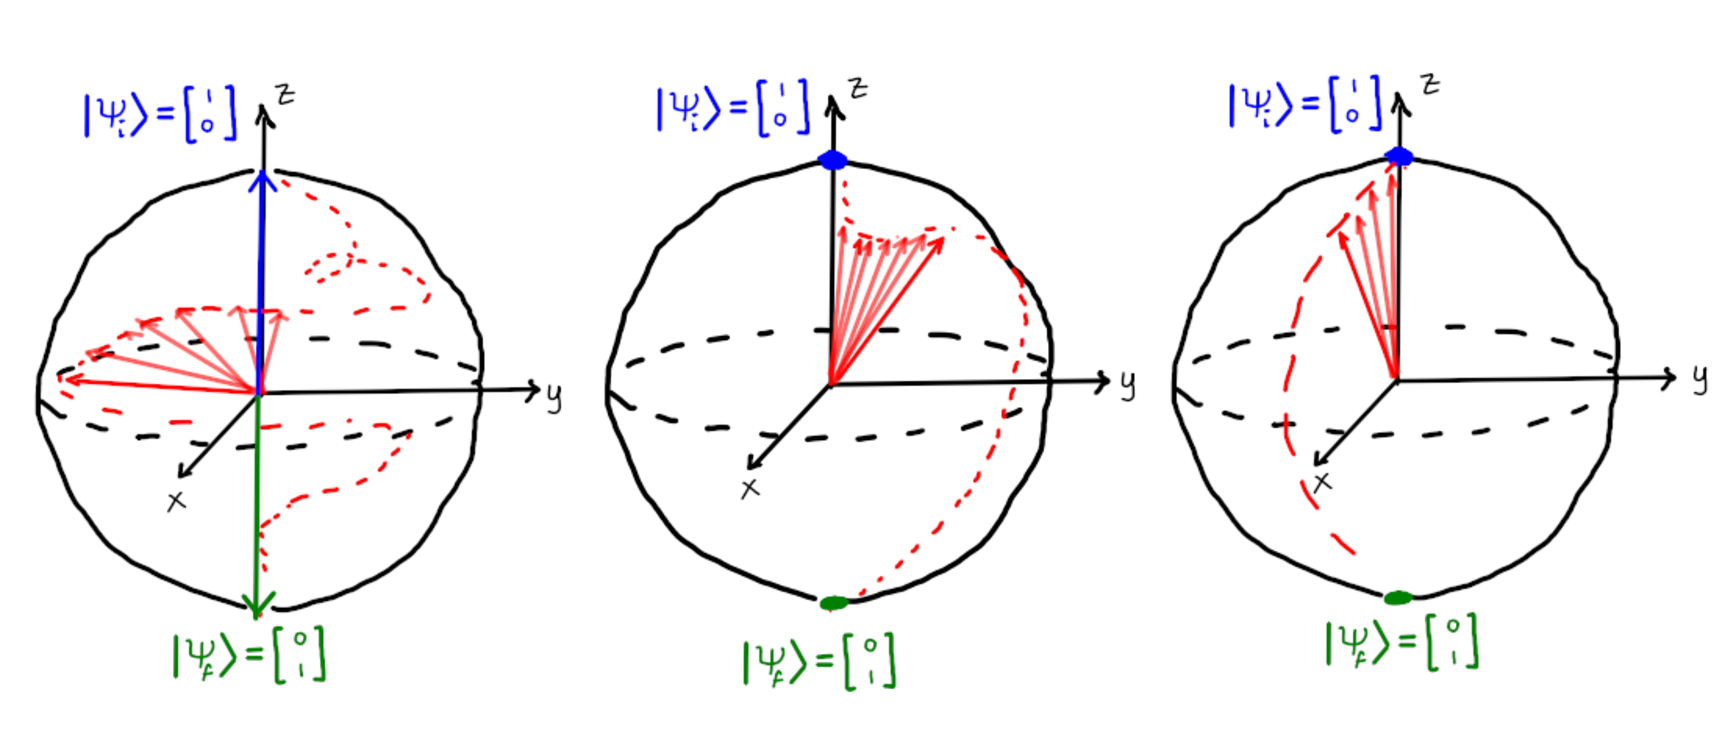
\includegraphics[width=\linewidth]{Bloch_spheres.pdf}
% \captionof{figure}{}
% \label{fig:bloch}
% \end{Figure}


% %visualising my project
% \begin{Figure}
% \centering
% 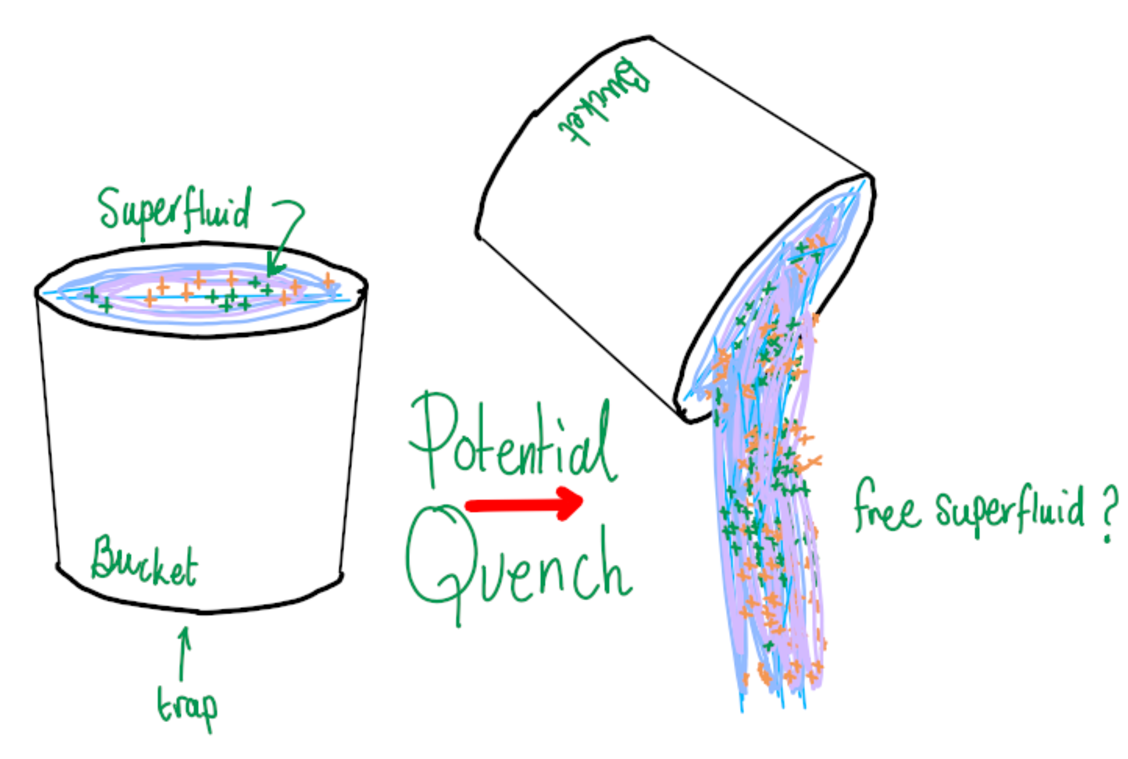
\includegraphics[width=.6\linewidth]{physical_bucket.pdf}
% \captionof{figure}{}
% \label{fig:}
% \end{Figure}


% %Investigating a potential quench 
% \begin{Figure}
% \centering
% 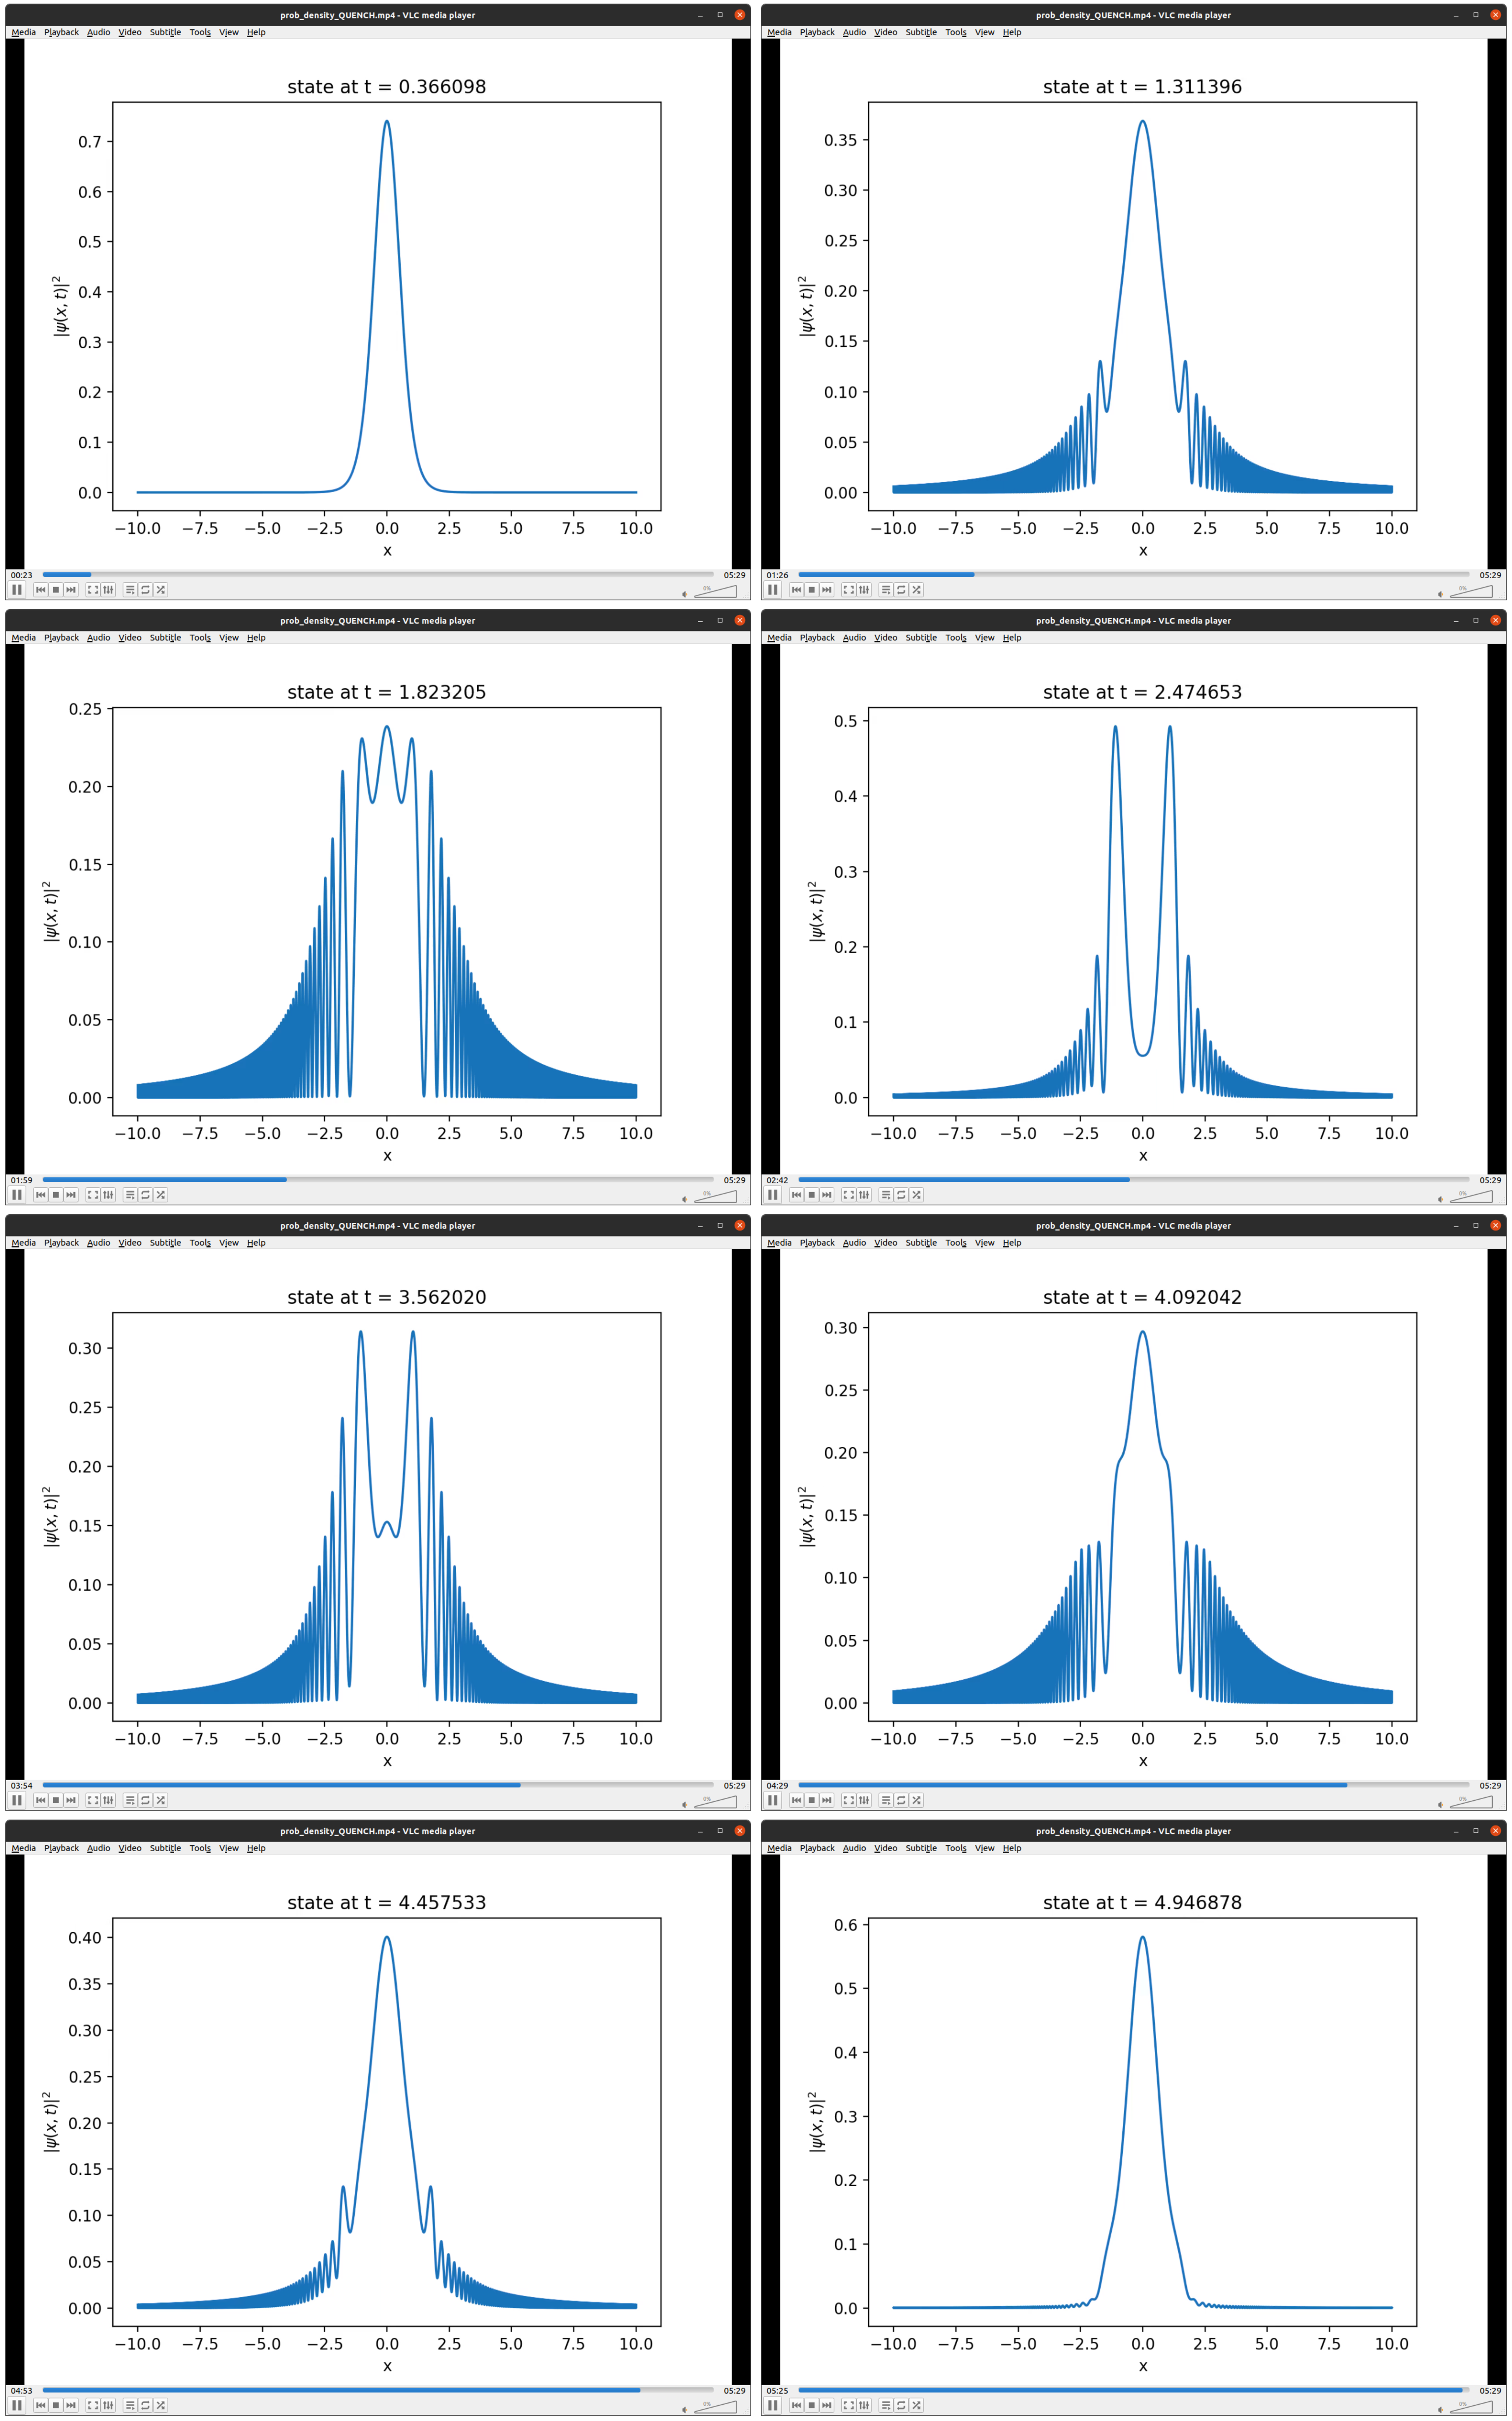
\includegraphics[width=.8\linewidth]{probability_density_in_negquartic.pdf}
% \captionof{figure}{}
% \label{fig:}
% \end{Figure}




%%%%%%%%%%%%%%%%%%%%%%%%%%%%%%%%%%%%%%%%%%%%%%%
\chapter{Conclusion}\label{Conclusion}

% Exact \PT-symmetry of Hamiltonians is understood to be equivalently useful at describing quantum mechanical systems as the mathematical postulate of Dirac Hermiticity



% \PT\:symmetry is a dynamic property of a Hamiltonian $(\hat{H})$, in the sense that it is strongly dependent on the boundary conditions implemented on the eigenfunctions of $\hat{H}$.

%


%%%%%%%%%%%%%%%%%%%%%%%%%%%%%%%%%%%%%%%%%%%%%%%
\chapter{Appendix}\label{appendix}

\section*{Bi-orthogonality and completeness}\label{}
In the case of a \PT-symmetric Hamiltonian $\tilde{H}$, it is possible for two (or more) complex eigenvalues to cross. At the crossing point the eigenvalues are degenerate and this is accompanied by the coalescence of the eigenstates of $\tilde{H}$. If eigenstates of $\tilde{H}$ become degenerate this implies that they lose completeness\cite{Brody_2013}. This special situation is associated with a branch point in the complex energy plane and is commonly termed an ``exceptional point"\cite{Moiseyev}. Moreover, sufficiently close to the branch point the eigenfunctions of the coalescing eigenvalues are nearly self-orthogonal.

We need completeness and closure relations in order to develop, for example, perturbation theory and scattering theories for non-Hermitian Hamiltonians and in order to be able to solve the Schrödinger equation by numerical methods\cite{Moiseyev}.

Suppose that a diagonalizable non-Hermitian Hamiltonian $\tilde{H}$ has a discrete spectrum and it commutes with the \PT\:operator.  This means that  $\tilde{H}$ has unbroken \PT-symmetry. A Hilbert space $\mathcal{H}$ spanned by the eigenvectors of $\tilde{H}$ exists, but because $\tilde{H}$ is non-Hermitian --with respect to the standard inner product of $\mathcal{H}$-- the time evolution generated by $\tilde{H}$ will not be unitary\cite{Mostafazadeh}. Nevertheless, as explained in section \ref{CC}. For the assumed $\tilde{H}$ above it is possible to construct a different complete positive-definite inner product by constructing and using the antisymmetric \CC\:operator that corresponds to $\tilde{H}$.

The assumed diagonalizability condition of $\tilde{H}$ may be viewed as a physical requirement without which an energy eigenbasis would not exist. To our knowledge all known non-Hermitian Hamiltonians that are used in physical applications are diagonalizable and therefore admit a complete \emph{bi-orthonormal} set of eigenvectors. This set of bi-orthonormal eigenvectors is $\{(\ket{\psi_{n}, a}, \ket{\phi_{n}, a})\}$ and will satisfy the following defining relations\cite{Pseudo-HermiticityIII}
\begin{align}
\tilde{H}\ket{\psi_{n}, a} = E_{n}\ket{\psi_{n}, a},\quad\tilde{H^{\dagger}}\ket{\phi_{n}, a} &= E^{*}_{n}\ket{\phi_{n}, a},\\
\nonumber\\
\braket{\phi_{m}, b|\psi_{n}, a} = \delta_{mn}\delta_{ab}&,\\
\nonumber\\
\sum^{}_{n}\sum_{a=1}^{d_n}\ket{\psi_{n}, a}\bra{\phi_{n}, a} = \hat{\mathbb{I}}&\\
\tilde{H} = \sum^{}_{n}\sum_{a=1}^{d_n}E_{n}\ket{\psi_{n}, a}\bra{\phi_{n}, a},\quad\tilde{H^{\dagger}} &= \sum^{}_{n}\sum_{a=1}^{d_n}E_{n}^{*}\ket{\phi_{n}, a}\bra{\psi_{n}, a}
\end{align}
where $n$ and $a$ are the spectral degeneracy levels, $d_n$ is the degree of degeneracy of $E_n$ and $\hat{\mathbb{I}}$ is the identity operator\cite{Pseudo-HermiticityIII}.

%%%%%%%%%%%%%%%%%%%%%%%%%%%%%%%%%%%%%%%%%%%%%%%%%%%%%%%%%%%%%%%%%%%%%%%%%%%%%%%%%
\section*{Equivalent Hamiltonians with distinct symmetries}\label{}
In parallel to the work of Bender is the research of Mostafazadeh who introduced the notion of pseudo-Hermiticity in \cite{Mostafazadeh}. A Hamiltonian is said to be pseudo-Hermitian with respect to a positive-definite, Hermitian operator $\eta$ if it satisfies
\begin{equation}\label{eq:2.1}
\tilde{H}^{\dagger}  = \eta^{-1}\tilde{H}\eta.
\end{equation}
In the case of Hamiltonians with \PT-symmetry, the role of $\eta$ is played by the combines action of \PP\:and \CC. A convenient way to write the \CC\:operator was proposed in \cite{Bender_2006} 
\begin{equation}\label{eq:2.2}
\mathcal{C} = e^{Q}\mathcal{P} = \eta^{-1}\mathcal{P} ,
\end{equation}
here $Q$ is an antisymmetric Hermitian operator. Mostafazadeh \cite{Mostafazadeh2} has shown that the square root of the positive-definite Hermitian operator $\eta = e^{-Q}$ can be used to transform any non-Hermitian Hamiltonian with unbroken \PT-symmetry into a spectrally equivalent Hermitian Hamiltonian by means of a unitary ``similarity transformation"\cite{PTvsDH}\cite{Jones_2005}. The transformation is as follows, the invertible operator $\rho = \sqrt{\eta}$ acts on the non-Hermitian \PT-symmetric Hamiltonian $\tilde{H}$ and returns an equivalent Hermitian Hamiltonian $\hat{H}$
\begin{equation}\label{eq:2.3}
\hat{H} = \rho^{-1}\tilde{H}\rho = e^{-Q/2}\tilde{H}e^{Q/2}.
\end{equation}
To verify that the similar Hamiltonian $\hat{H}$ is Hermitian we take the Hermitian conjugate of $\hat{H}$
\begin{align}\label{eq:2.4}
\hat{H}^{\dagger} &= (e^{-Q/2}\tilde{H}e^{Q/2})^{\dagger}\nonumber,\\
& = e^{Q/2}\tilde{H}^{\dagger}e^{-Q/2},
\end{align}
If we ``swap" Hermiticity: $\tilde{H}^{\dagger}$ in \ref{eq:2.4} for \PT-symmetry, and we use equation \ref{eq:12}
\begin{align}\label{eq:2.5}
\hat{H}^{\dagger} &= e^{Q/2}\mathcal{P}\tilde{H}\mathcal{P}^{-1}e^{-Q/2}\nonumber,\\
&= e^{-Q/2}\mathcal{C}\tilde{H}\mathcal{C}^{-1}e^{Q/2},
\end{align}
Finally we recall that \CC\:and $\tilde{H}$ commute
\begin{equation}\label{eq:2.6}
\hat{H}^{\dagger} = e^{-Q/2}\tilde{H}e^{Q/2} = \hat{H}.
\end{equation}
Mostafazadeh \cite{Mostafazadeh}, conjectures that because \CPT-symmetry satisfies the postulates of quantum mechanics --whilst only ``swapping" the Hermiticity of a Hamiltonian by \CPT-symmetry-- then this must mean that non Hermitian \CPT-symmetric theories are equivalent to certain non local Hermitian field theories. This kind of transformation is explored in references \cite{Mostafazadeh},\cite{EquivalentHH},\cite{Pseudo-HermiticityIII},\cite{Jones_2005},\cite{taleof2potentials}.
In general this transformation is extremely complicated and so it is quite impractical to perfom. Hence, while the mapping from \PT-symmetric to Hermitian Hamiltonians is of great theoretical interest, it does not have much practical value\cite{MakingSense}. Another important fact is that this kind of transformation is a similarity and not a unitary transformation. Thus, while the eigenvalues of both Hamiltonians are identical, the relationships between
vectors are changed; pairs of vectors that are orthogonal are mapped into pairs of vectors that are not orthogonal\cite{MakingSense}\cite{Bender_2007}.

\section*{One-to-one equivalence:\\ PT-symmetric and Hermitian quantum properties}\label{}

In the case of unbroken \PT-symmetry of a Hamiltonian $\tilde{H}$ with eigenfucntions $\psi_n$ then the \PT\:operator eigenfunctions are: $\chi_{n}(x) = e^{-i\alpha/2}\psi_n(x)$\\

{\renewcommand{\arraystretch}{2}
\noindent\begin{tabularx}{1.1\textwidth} { 
  | >{\raggedright\arraybackslash}X 
  | >{\raggedright\arraybackslash}X 
  | >{\raggedright\arraybackslash}X | }
 \hline
  \textbf{Properties} 
  & \textbf{Hermitian} 
  & \textbf{\PT-symmetry}\newline \small{(unbroken)} \\
   \hline
  Eigenvalues \newline and Eigenstates
  & $\hat{H}\ket{\psi_n} = E_n \ket{\psi_n}$ 
  & $\tilde{H}\ket{\psi_n} = E_n \ket{\psi_n}$, $\bra{\phi_n}\tilde{H}^{\dagger} = \bra{\phi_n}E_{n}^{*}$\vspace{0.001cm} \\
  \hline
  Inner product \newline \tiny{(ignoring degenerate spectra)}
  & $\braket{\psi|\phi} = (\ket{\psi})^{\dagger} \cdot \ket{\phi}$
  & $\left(\psi|\phi\right) = (\mathcal{CPT}\ket{\psi})^{T} \cdot \ket{\psi}$ \\
  \hline
  Orthonormality of states 
  & $\braket{\psi_n|\psi_m} = \delta_{mn}$ 
  & $\left(\psi_n|\psi_m\right) = \delta_{mn}$\\
  \hline
  Completeness of states 
  & $\sum\limits_{n = 0}^{\infty} [\psi(x)]^{*} \psi(y) = \delta(x-y)$
  & \begin{small}{$\sum\limits_{n = 0}^{\infty} (-1)^{n} \chi_n(x) \chi_n(y) = \delta(x-y)$}\end{small}\\
  \hline
  Hamiltonian, Greens \newline and zeta functions 
  & \small{$H(x,y) = \sum\limits_{n = 0}^{\infty} E_n [\psi_n(x)]^{*}\psi_n(y)$, 
  \newline $G(x,y) = \sum\limits_{n = 0}^{\infty} \frac{1}{E_n} [\psi_n(x)]^{*}\psi_n(y)$,
  \newline $\int dx G(x,x) =  \sum\limits_{n = 0}^{\infty} \frac{1}{E_n}$}
  & \small{$H(x,y) = \sum\limits_{n = 0}^{\infty}(-1)^{n} E_n \chi_n(x)\chi_n(y)$, \newline $G(x,y) = \sum\limits_{n = 0}^{\infty} \frac{(-1)^n}{E_n}\chi_n(x)\chi_n(y)$, \newline }\\

  \hline
  Time evolution
  & $\hat{U} = e^{-i\hat{H}t/\hbar}$
  & $\hat{U} = e^{-i\tilde{H}t/\hbar}$\\
  \hline
\end{tabularx}
}
%%%%%%%%%%%%%%%%%%%%%%%%%%%%%%%%%%%%%%%%%%%%%%%


\section*{Stokes wedges and boundary conditions}\label{}
% The class of \PT-symmetric Hamiltonians is larger than and includes Hermitian Hamiltonians because any real symmetric Hamiltonian is automatically \PT-symmetric\cite{MustaHbeHermitian}


% This means the domain of integration, which makes
% the eigenvalue problem of the non-Hermitian Hamilto-
% nian operator in (1) in position space well defined for the
% asymptotic boundary condition Φ(z) → 0 exponentially
% for |z| → ∞ is any path in the complex z-plane which re-
% mains inside the wedges and when it approaches
% complex infinity\cite{Faria1}.

\bibliographystyle{unsrturl_mod}
\bibliography{mybib}

\end{document}